\documentclass{article}
\usepackage[utf8]{inputenc}
\usepackage[english]{babel}
\usepackage[]{amsthm} 
\usepackage[]{amssymb} 
\usepackage{amsmath}
\usepackage[nottoc]{tocbibind}
\usepackage{graphicx}
\usepackage{adjustbox}
\usepackage{float}

\usepackage{algorithm}
\usepackage{algpseudocode}


\title{Complex Networks: Midterm 1 - Q2}
\author{Alara Dirik}
\date\today

\begin{document}
\maketitle 
\newpage
\section*{Introduction}
The aim of this project is to experiment with the SIR epidemic model and discover insights on how disease progresses in a small, tightly knit community with no random movements. The community is modeled as a regular, undirected and unweighted ring lattice network with {\it n} vertices and degree of {\it k}. 


\subsection*{Experimental Setup}
A SIR Model was implemented in Python to simulate how the epidemic unfolds with different infection rates $\beta$ up until the epidemic termination date. Number of nodes {\it n}/population, degree {\it k} and the recovery rate $\gamma$ were held constant with values of 5000, 4 and 7 (days) respectively, and $\beta$ values of 0.25, 0.50 and 0.75 were tested. \\

\noindent
Degree {\it k} is the number of first order neighbors each node has in the ring lattice network and can be interpreted as the number of direct contacts per individual/day. Unlike a random network where nodes might interact with different nodes over time, nodes in the ring lattice has direct contact only with their 1st degree neighbors at any time. The $\gamma$ parameter denotes the average time (usually in days) for infected individuals to recover in the SIR model. Since the SIR model does not assume reinfection, the epidemic termination date is considered as the day no individual is infected. \\

\noindent
The pseudo code of the experiments is given in Figure \ref{fig_pseudocode}.
\begin{figure}[!htb]
\begin{center}
\scalebox{0.94}{\small
\framebox[3.53in]{
\begin{minipage}[t]{3.5in}

\begin{algorithmic}[1]
\State Input: {\it n}, {\it k}, $\gamma$, $\beta$
\State Output: Epidemic simulation

\State Initialize ring lattice with {\it n}, {\it k} parameters
\State Initialize epidemic by assigning a random node as infected and the rest as susceptible

\While { number of susceptible nodes != 0}
	\For { $i \gets 1$ to number of infected nodes $node_i$}
	    \State Assign $node_{i}$ as recovered with probability $1/\gamma$
		\State Retrieve 1st order neighbors of $node_i$
		\For { $j \gets 1$ to degree {\it k}}
    		\If { $node_{ij}$ is susceptible } 
    			\State Assign $node_{ij}$ as infected with probability $\beta$
    		\EndIf
		\EndFor
	\EndFor
\EndWhile
\end{algorithmic}
\end{minipage}
}
}
\end{center}
%\vspace{-4mm}
\caption{Pseudo code of the SIR model - ring lattice simulation.}
\label{fig_pseudocode}
\end{figure}

\subsection*{Results}
The effect of $\beta$ value on epidemic spread rate was evaluated by running 100 realizations with the same configuration for each of the $\beta$ values: 0.25, 0.5, 0.75. The average number of days to reach the maximum number of infections and the average number of days till epidemic termination are given in Table \ref{results}.

\begin{table} [H]
\centering
\begin{tabular}{ |p{2cm}|p{3cm}|p{3cm}| }
\hline
\multicolumn{3}{|c|}{Simulation results} \\
\hline
Beta & Days till Peak & Days till Term. \\
\hline
0.25 & $11.69$ & $39.81$ \\
0.50 & $25.36$ & $90.47$ \\
0.75 & $19.2$ & $86.23$ \\
\hline
\end{tabular}
\caption{Simulation results for different beta values.}
\label{results}
\end{table} 

\noindent
The results show that epidemic is terminated quickly when the $\beta$ value is lowest at 0.25 and takes the longest to peak and terminate with the $\beta$ value 0.5. Given that infected nodes only have contact with their {\it k} first order neighbors and take on average $\gamma$ days to recover, there is a high possibility of infected nodes recovering without infecting anyone for low $\beta$ and $\gamma$ values. Additionally, the epidemic can be prevented if patient zero recovers without infecting anyone. \\

\noindent
Sample simulation plots given in Figure 2\ref{fig:samples} illustrate that a very large percentage of the population never gets infected for $\beta$ values of 0.25 and 0.5. Furthermore, the limited and structured contact between the nodes act as barrier against the spread of the disease, allowing the disease to slowly die off while effecting a minimal number of people. Despite still effecting a small fraction of the population, an epidemic with the $\beta$ value 0.5 lasts over twice as long as an epidemic with a $\beta$ value 0.25. On the other hand, a $\beta$ value of 0.75 reportedly gives the epidemic spread a strong boost by increasing the chances of an infected node infecting its neighbors before recovering. Thus, the whole population becomes infected at one point for large $\beta$ values. \\

\begin{figure}[H]
\begin{adjustbox}{max width=1.2\linewidth,center}
\centering
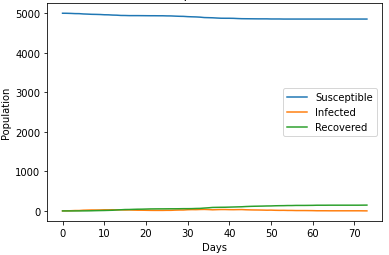
\includegraphics[width=.4\textwidth]{images/beta025.png}\hfill
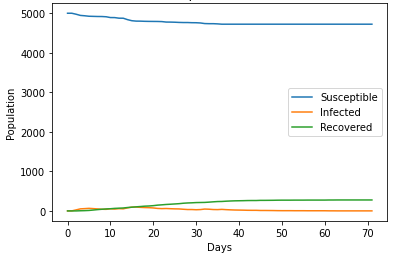
\includegraphics[width=.4\textwidth]{images/beta050.png}\hfill
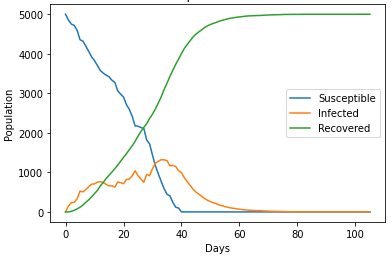
\includegraphics[width=.4\textwidth]{images/beta075.png}
\end{adjustbox}
\caption{Epidemic realizations for beta values 0.25, 0.50 and 0.75 respectively.}
\end{figure} \label{fig:samples}

\end{document}